\documentclass[final,3p,times,onecolumn]{elsarticle}
\usepackage{amssymb}
\usepackage[fleqn]{amsmath}
\usepackage{graphicx}
\usepackage{footnote}
\usepackage{graphicx}
\usepackage{array,booktabs}
\usepackage{algorithmic,algorithm}
\usepackage{pbox}
\usepackage{enumitem}
\usepackage{color}
\usepackage{hyperref}
\setlength\parskip{\baselineskip}
%\setlength{mathindent}{0pt}
\setlength\parindent{0pt}
\journal{MPhil in Scientific Computing}

\begin{document}

\begin{frontmatter}
\begin{abstract}
In this short report we try to quantify the importance of feature A for Higgs classification in the Kaggle dataset. The approach used here is that of Gaussian Kernel Support Vector machines to auto-classify Higgs collisions from other background processes. Feature \textbf{A}, an analytically constructed likelihood value was proposed by Dr. Christopher Lester at the Cavendish Laboratory, High Energy Physics group. We use a set of pre-optimized parameters proposed in \cite{Vid} and test the AMS performance of classifying the collisions under a model trained on a set of features which includes feature A and one that excludes feature A.

\end{abstract}
\title{HiggsML Challenge - Quantifying feature A}
\author{Vidhi Lalchand}
\address{Cavendish Laboratory, Department of Physics, J J Thomson Avenue, Cambridge. CB3 0HE}
\end{frontmatter}

\section{Feature-class correlation}


Since the class variable is dichotomous, $y_{i} \in \{0,1\} \forall i$, the feature vs. class correlation is computed using the point-biserial correlation. This is mathematically equivalent to the Pearson correlation for computing correlations between one continuous and one dichotomous variable. The point-biserial correlation was computed between each feature and the binary class variable. It is computed as, 

\begin{equation}
r_{pb} = \dfrac{M_{1} - M_{0}}{s_{n}}\sqrt{\dfrac{n_{1}n_{0}}{n^2}}
\end{equation}
\\

where $M_{0}$ and $M_{1}$ are the mean values of the feature for the background and signal class. $s_{n}$ is the inter-class standard deviation of the feature, $n_{0}$ and $n_{1}$ represent the count of samples in the background and signal class and $n$ is the overall count. From figure \ref{biserial} it is apparent that the derived features showed higher correlation with the class label than the primary features. Visually observing the distribution of features with high point biserial correlation to each class label gives some insight \ref{dists_1} \ref{dists_2}. 
 
\begin{figure*}
\hspace{1.8cm}
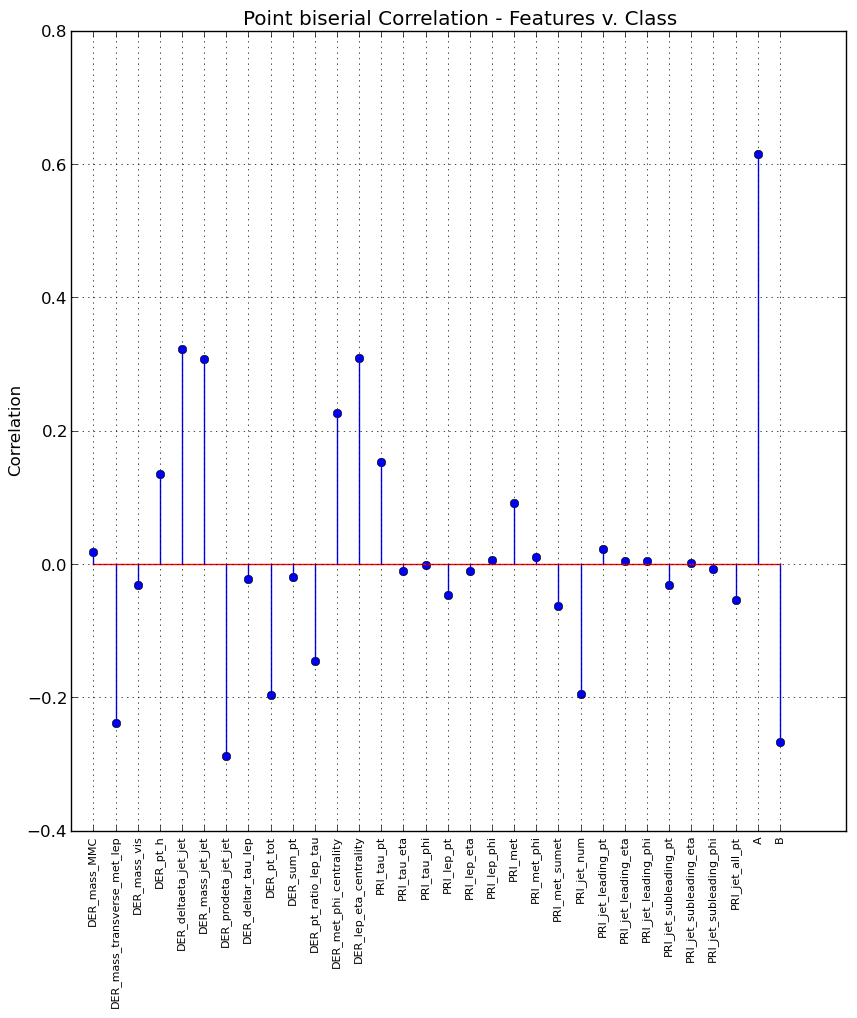
\includegraphics[scale=0.6]{Images/BiSerialCorr.png}
\caption{The figure shows the strength of correlation of derived features (DER\_$*$) over the primary features (PRI\_$*$). Derived jet features showed higher correlation and analytically derived feature A and B showed higher correlation to any of the primary features.}
\label{biserial}
\end{figure*}



\begin{figure*}
\hspace{-0.9cm}
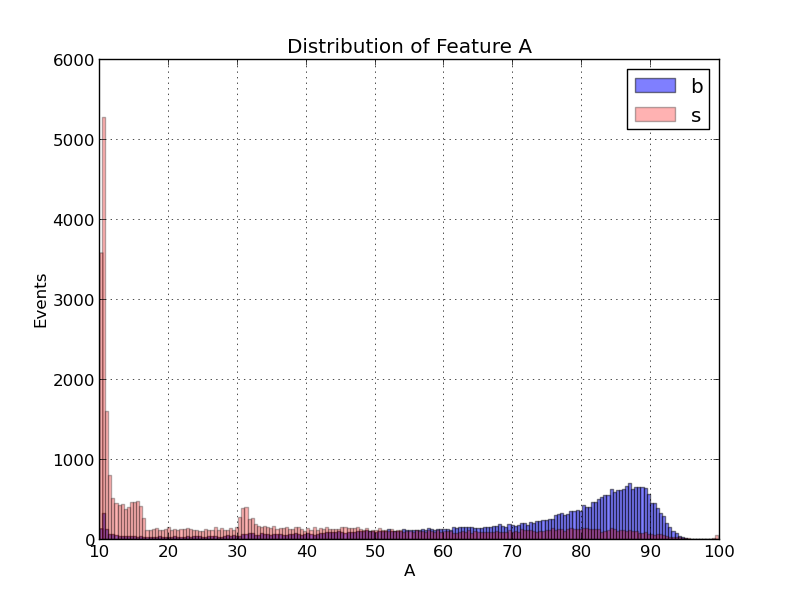
\includegraphics[scale=0.5]{Images/A_dist.png}
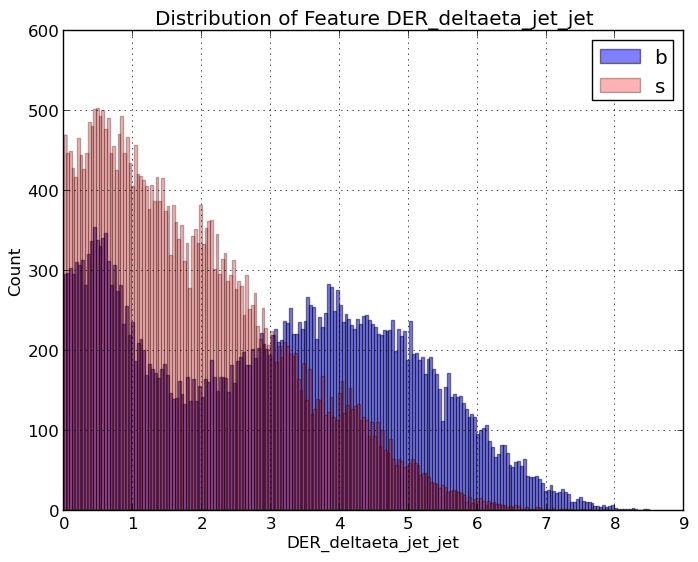
\includegraphics[scale=0.5]{Images/DER_deltaeta_jet_jet_Hist.png}
\caption{Distribution of Features by class breakdown}
\label{dists_1}
\end{figure*}

\begin{figure*}
\hspace{-0.5cm}
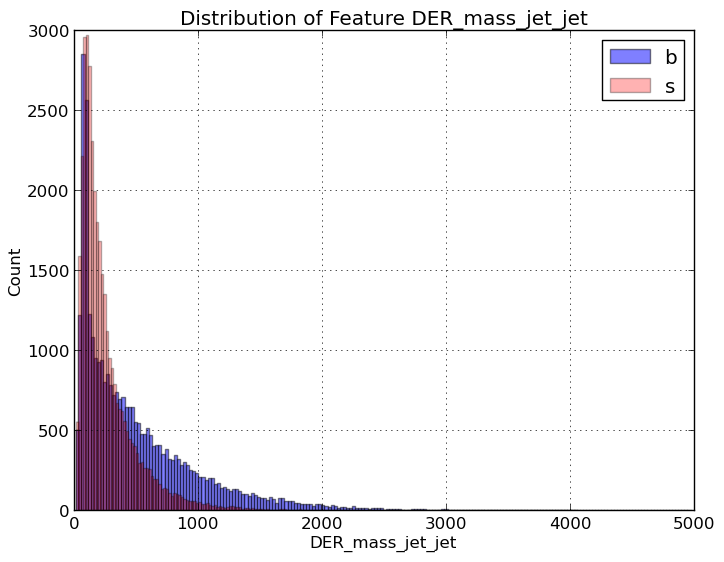
\includegraphics[scale=0.5]{Images/DER_mass_jet_jet_Hist.png}
\hspace{4mm}
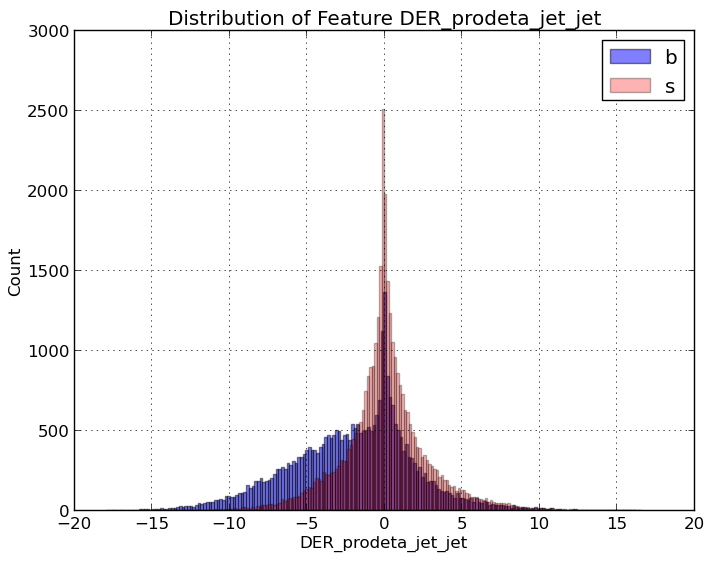
\includegraphics[scale=0.5]{Images/DER_prodeta_jet_jet_Hist.png}
\caption{Distribution of Features by class breakdown}
\label{dists_2}
\end{figure*} 

\section{AMS results}
 
There were 250,000 rows in the complete data set. We dropped rows which contain missing values (-999.0) in any of the features. The data set without any missing value tags had 68114 rows. We split this condensed data set into a training and test set in the ratio of 80:20.   

\section{Challenges in measuring the AMS difference}

Firstly, the optimal parameters in the presence of feature A are different to the ones obtained when optimized without feature A. As a first step, we obtain two optimized models, one optimized in the presence of feature A and the other optimized without feature A. Further, the AMS value is sensitive to the choice of threshold and in order to account for this, we visualize AMS curves for both the models across a range of thresholds. The final training set which is fed to the SVM is constructed by sampling the original training set, hence repeated runs of the learning algorithm gave different AMS scores. In order to account for variational effects of sampling, we introduce error bars on the AMS score at each threshold centered on the mean AMS score computed by averaging the outcome of 10s0 iterations of the sampling and model fitting step. The AMS curves obtained for the two models are given in fig \ref{ams_compare}.

\begin{figure}
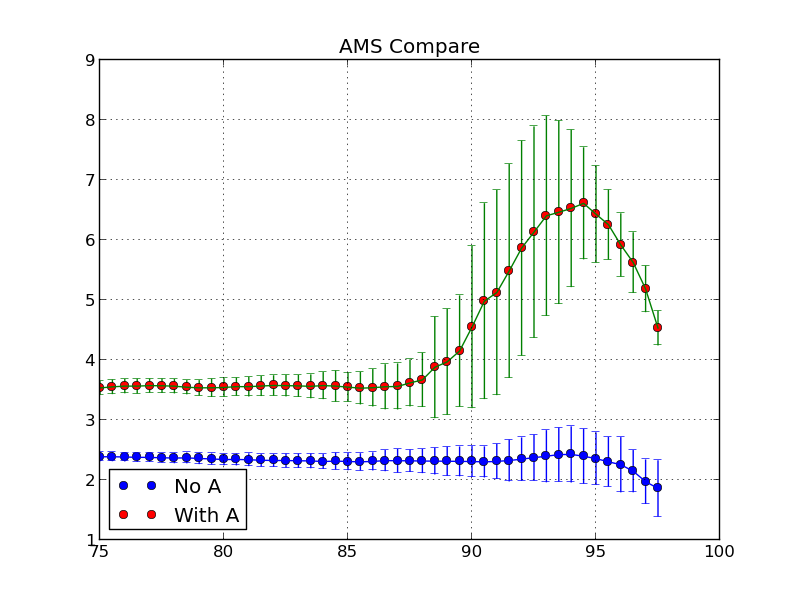
\includegraphics[scale=0.8]{Images/AMS_compare.png}
\caption{AMS curves with and without feature A, x-axis measures the rejection threshold (\%) and y-axis shows the AMS score}
\label{ams_compare}
\end{figure}
  

\section{Summary}

The inclusion of feature A in the dataset improves the AMS score by a significant margin. The improvement in score can be quantified by computing the difference between the mean AMS scores across a range of thresholds. For instance, the improvement in score in the threshold range of 83 to 87 is 0.98 $\pm$ 0.7. The important point to note is that we consider a relatively small fraction of the full dataset in training and testing the model. At the expense of compute time, it is possible to test how the model fares by taking into account the full training dataset of 250,000 samples by imputing the missing values either by using mean or median and testing on a larger sample of data.

\section*{References}
\bibliography{References_A} 
\bibliographystyle{elsart-num-names.bst}

\end{document}
